\chapter{Аналитический раздел}

В данном разделе будет представлено описание предметной области и описаны особенности реализации стеков на списке и на массиве. Также будет описано условие и техническое задание лабораторной работы.

\section{Сведения о стеке}

Стек – это последовательный список с переменной длиной, в котором включение и 
исключение элементов  происходит  только с одной стороны  –  с его вершины. Стек 
функционирует по принципу: последним пришел –  первым ушел, \textit{Last In  –  First  Out} 
\textbf{(LIFO)}. 

Программная реализация стека возможна на основе различных структур данных, 
например,  с  использованием  статических  или  динамических  одномерных  массивов 
(векторов) и линейных списков.  

При работе со стеком доступен только его верхний элемент, который  адресуется 
специальным указателем  стека PS  (Pointer  Stack). Причем классическая реализация стека 
предполагает,  что  просмотреть  содержимое  стека  без  извлечения  (удаления)  его 
элементов невозможно.  

При работе со стеком необходимо отслеживать возникновение таких аварийных 
ситуаций, как попытки исключения элемента из пустого стека и переполнения стека. При 
реализации стека в  виде вектора переполнение возникает  вследствие ограниченности 
объема памяти, выделяемой под размещение массива. Однако, даже если стек реализован 
на основе динамического списка, его размер также не безграничен, он ограничен объемом 
доступной  программе  оперативной  памяти  (обычно  он  ограничивается  небольшим 
объемом,  256,  512  КБ).  Для  отработки  указанных  аварийных  ситуаций  в  программе 
должны быть предусмотрены дополнительные проверки на пустоту и переполнение стека 
и выдача соответствующих сообщений. 

\section{Реализации стека}

Ниже представлены основные варианты реализации стека на основе массива и списка.

\subsection{Реализация стека в виде массива}

Реализация стека в виде массива. Если стек реализован в виде статического или 
динамического массива (вектора), то для его хранения обычно отводится непрерывная 
область памяти ограниченного размера, имеющая нижнюю и верхнюю границу. Перед 
началом работы указатель стека PS находится ниже левой (нижней) границы массива. При 
включении первого элемента в стек указатель PS устанавливается на начало массива и по 
адресу первого элемента размещается записываемое значение. При попытке добавить в 
стек каждый последующий элемент сначала происходит смещение указателя на длину 
типа  данных  (т.е.  он  перемещается  к  следующему  элементу  массива),  а  затем  – 
размещение значений элементов по этим адресам. Если указатель выходит за верхнюю 
границу массива, то это признак того, что стек переполнен. При исключении элемента из 
стека сначала считываются данные, а затем  происходит перемещение указателя PS  к 
предыдущему элементу. Если указатель стека выходит за нижнюю границу массива, то 
стек пуст.

\subsection{Реализация стека в виде списка}

Реализация стека в виде списка. До начала работы указатель стека показывает на 
нулевой, физически отсутствующий адрес (т. е.  указатель  -  пустой). При включении 
элемента  в  стек  сначала  происходит  выделение  области  памяти,  адрес  которой 
записывается в указатель стека, а затем по значению этого указателя в стек помещается 
информация.  

При исключении  элемента сначала по указателю стека считывается информация об 
исключаемом элементе, а затем указатель смещается к предыдущему элементу. После 
чего освобождается память, выделенная под элемент. Если указатель имеет значение 
нулевого адреса, то стек пуст.  

При физической реализации стека в виде односвязного линейного списка дескриптор 
будет  отличаться  отсутствием  верхней  границы  стека.  В  этом  случае  объем  стека 
ограничивается только объемом доступной оперативной памяти.

\section{Условие задачи}

Создать  программу  работы  со  стеком, 
выполняющую  операции  добавление, 
удаления  элементов  и  вывод  текущего 
состояния стека. Реализовать стек: 
а)  массивом;  б)  списком.  Все  стандартные 
операции со стеком должны быть оформлены 
подпрограммами.  При  реализации  стека 
списком  в  вывод  текущего  состояния  стека 
добавить просмотр адресов элементов стека и 
создать  свой  список  или  массив  свободных 
областей (адресов освобождаемых элементов) 
с выводом его на экран.

\section{Техническое задание}

При реализации стека массивом располагать два 
стека в одном массиве. Один стек располагается в 
начале массива и растет к концу, а другой 
располагается в конце массива и растет к началу. 
Заполнять и освобождать стеки произвольным 
образом с экрана. Элементами стека являются  
вещественные числа. Списком реализовать один 
стек.

\section{Вывод}

В данном разделе были представлены основные теоритические сведения о стеках и их реализациях. Также было сформулировано техническое задание.

\chapter{Конструкторский раздел}

В данном разделе описаны используемые структуры данных, а также представлены схемы алгоритмов и подсчет затрат памяти под хранение стеков.

\section{Схемы алгоритмов}

Ниже, на рисунке \ref{alg:lpush}, представлена cхема алгоритма вставки элемента в стек, представленный списком.

\begin{figure}[h]
	\centering
	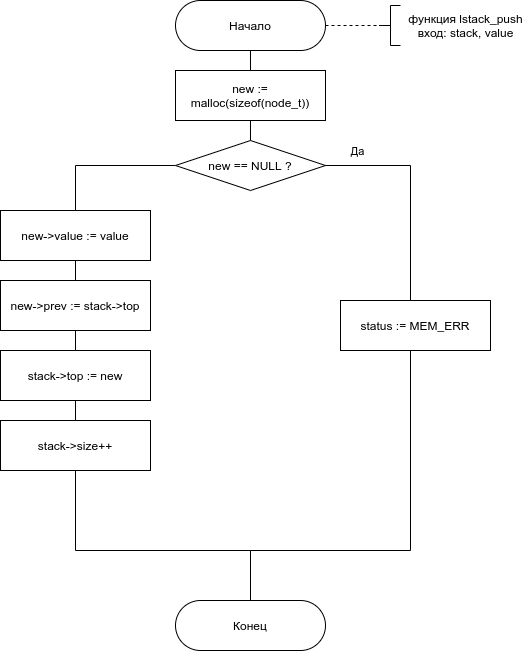
\includegraphics[width=0.6\linewidth]{img/algo-lstack_push.png}
	\caption{схема алгоритма вставки элемента в стек-список.}
	\label{alg:lpush}
\end{figure}

\clearpage

Ниже, на рисунке \ref{alg:lpop}, представлена схема алгоритма удаления элемента из стека, представленного списком.

\begin{figure}[h]
	\centering
	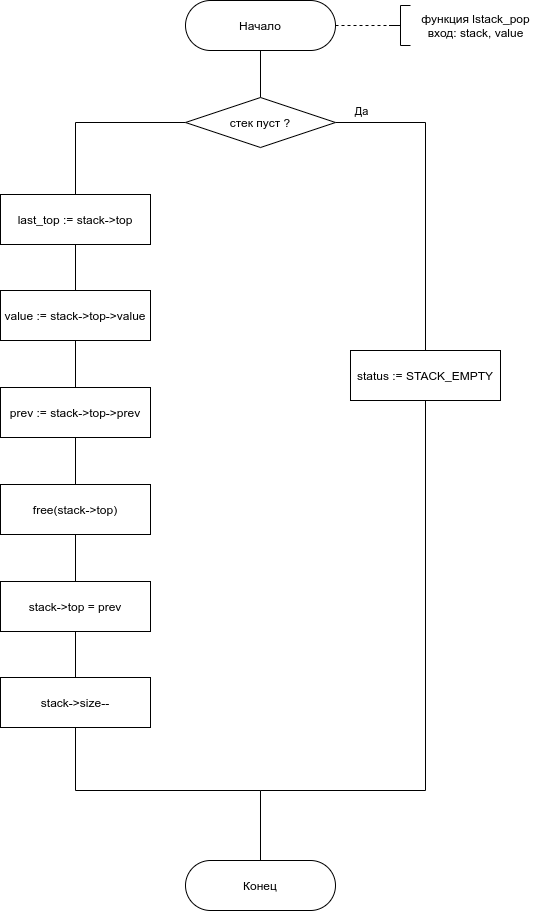
\includegraphics[width=0.6\linewidth]{img/algo-lstack_pop.png}
	\caption{схема алгоритма удаления элемента из стека-списка.}
	\label{alg:lpop}
\end{figure}

\clearpage

Ниже, на рисунке \ref{alg:apush-l}, представлена схема алгоритма вставки в нижний стек, хранящийся в массиве.

\begin{figure}[h]
	\centering
	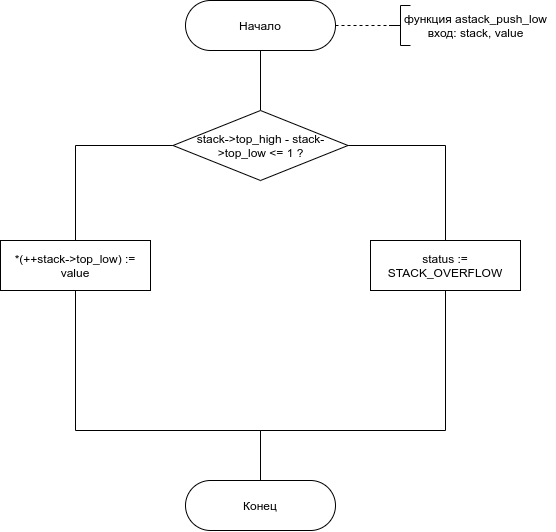
\includegraphics[width=0.5\linewidth]{img/algo-astack_push_low.png}
	\caption{схема алгоритма вставки элемента в нижний стек-массив.}
	\label{alg:apush-l}
\end{figure}

Ниже, на рисунке \ref{alg:apush-h}, представлена схема алгоритма вставки в нижний стек, хранящийся в массиве.

\begin{figure}[h]
	\centering
	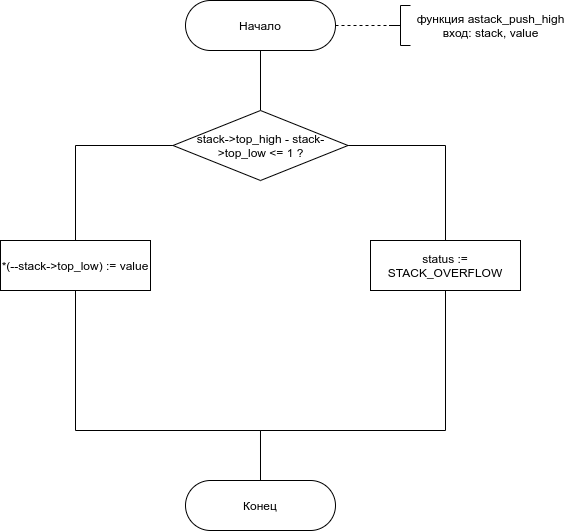
\includegraphics[width=0.5\linewidth]{img/algo-astack_push_high.png}
	\caption{схема алгоритма вставки элемента в верхний стек-массив.}
	\label{alg:apush-h}
\end{figure}

\clearpage

Ниже, на рисунке \ref{alg:apop-l}, представлена схема алгоритма удаления из нижнего стека, хранящегося в массиве.

\begin{figure}[h]
	\centering
	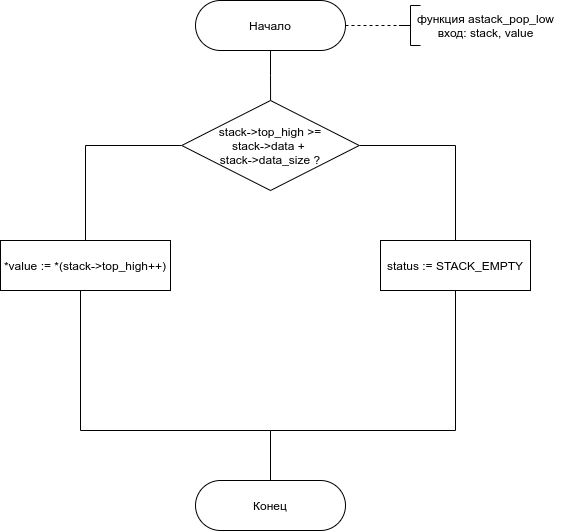
\includegraphics[width=0.5\linewidth]{img/algo-astack_pop_high.png}
	\caption{схема алгоритма удаления элемента из нижнего стека-массива.}
	\label{alg:apop-l}
\end{figure}

Ниже, на рисунке \ref{alg:apop-h}, представлена схема алгоритма удаления из верхнего стека, хранящегося в массиве.

\begin{figure}[h]
	\centering
	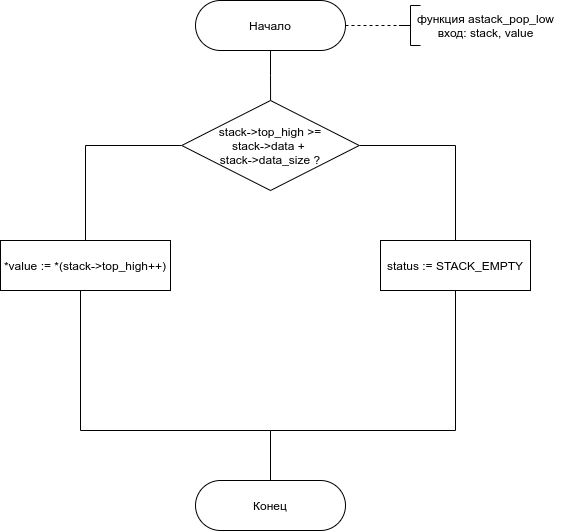
\includegraphics[width=0.5\linewidth]{img/algo-astack_pop_high.png}
	\caption{схема алгоритма удаления элемента из верхнего стека-массива.}
	\label{alg:apop-h}
\end{figure}

\clearpage

\section{Описание структур данных}

Ниже представлены листинги кодов используемых в ПО структур данных.

\begin{lstlisting}[language=C,caption=Cтек на списке.]
#define UNBOUND 0       // Если стек, ограничен только объемом оперативной памяти
						// то capacity = UNBOUND

typedef double data_t;

typedef struct node
{
	struct node *prev;  // Предыдущий (нижний) элемент
	data_t value;       // Значение текущего элемента
} node_t;

typedef struct
{
	node_t *top;        // Верхний элемент стека
	size_t size;        // Количество элементов в стеке
	size_t capacity;    // Вместимость стека
} lstack_t;
\end{lstlisting}

\begin{lstlisting}[language=C,caption=Стек на массиве]
typedef double data_t;

typedef struct
{
	data_t *data;       // Указатель на область памяти
	data_t *top_low;    // Указатель на верхний элемент нижнего стека
	data_t *top_high;   // Указатель на верхний элемент верхнего стека
	size_t data_size;   // Размер массива
} astack_t;
\end{lstlisting}

\begin{lstlisting}[language=C,caption=Коды ошибок]
#define SUCCESS         0   // Успешное выполнение
#define MEM_ERR         1   // Ошибка выделения памяти
#define INP_ERR         2   // Ошибка ввода
#define STACK_OVERFLOW  3   // Переполнение стека
#define STACK_EMPTY     4   // Пустой стек
#define STACK_INVALID   5   // Некорректный стек
\end{lstlisting}

\begin{lstlisting}[language=C,caption=Список адресов памяти для стека реализованного списком]
typedef struct mem_list
{
	const void *addr;       // Адрес памяти
	memstate_t state;       // Состояние адреса
	struct mem_list *next;  // Следующий адрес
} mem_list_t;

// Состояние адресов памяти
typedef enum
{
	UNUSED,     // Неиспользован
	USED,       // Использован
	REUSED      // Переиспользован
} memstate_t;
\end{lstlisting}

\section{Вывод}

В данном разделе были представлены схемы операций над стеками, а также приведены листинги кодов используемых структур данных.

\chapter{Технологический раздел}

В данном разделе будут представлены листинги кодов набора функций для работы со стеком, а также будет приведены требования к ПО и тестовые данные.

\section{Требования к ПО}

Ниже определены предъявляемые к ПО требования:

\begin{itemize}[$\bullet$]
	\item На вход программа получает пункт меню (от 0 до 8) и элемент для вставки при необходимости (вещественный);
	
	\textbf{значения пунктов меню: }
	\begin{itemize}
		\item 0 --- выход;
		\item 1 --- вывод стеков в массиве;
		\item 2 --- вывод стека на списке;
		\item 3 --- вставка в нижний стек в массиве;
		\item 4 --- вставка в верхний стек в массиве;
		\item 5 --- вставка в стек на спике;
		\item 6 --- удаление из нижнего стека в массиве;
		\item 7 --- удаление из верхнего стека в массиве;
		\item 8 --- удаление из стека на списке.
	\end{itemize}

	\textbf{При выборе пунктов меню 3, 4 или 5: программа получает на вход вещественное число}
	\item На выход программа подает текущее состояние стеков и адреса высвобождаемых/занятых/переиспользуемых списком областей памяти, а также время вставки элемента и используемую под каждую реализацию стека память.
\end{itemize}

\section{Набор функций для работы со стеком}

\subsection{Стек в виде списка}

Ниже представлен набор функций для работы со стеком на списке.

\begin{lstlisting}[language=C,caption=Набор функций для стека-списка.]
// Пустой список
lstack_t lstack_empty(size_t capacity);

// Освобождение памяти
void lstack_destroy(lstack_t *stack);

// Проверка на пустоту
bool lstack_is_empty(const lstack_t *stack);

// Вставка элемента
int lstack_push(lstack_t *stack, data_t value);

// Удаление элемента
int lstack_pop(lstack_t *stack, data_t *value);

// Вывод стека и адресов
void lstack_print(const lstack_t *stack);

// Память, занимаемая стеком
size_t lstack_sizeof(const lstack_t *stack);
\end{lstlisting}

\subsection{Стек в виде массива}

Ниже представлен набор функций для работы со стеками в массиве

\begin{lstlisting}[language=C,caption=Набор функций для стека-массива.]
// Непроинициализированный стек
astack_t astack_null(void);

// Пустой стек
astack_t astack_empty(size_t size);

// Освобождение памяти
void astack_destroy(astack_t *stack);

// Проверка на корректность
bool astack_is_valid(const astack_t *stack);

// Вставка в нижний (первый) стек
int astack_push_low(astack_t *stack, data_t value);

// Вставка в верхний (второй) стек
int astack_push_high(astack_t *stack, data_t value);

// Удаление из нижнего (первого) стека
int astack_pop_low(astack_t *stack, data_t *value);

// Удаление из верхнего (второго) стека
int astack_pop_high(astack_t *stack, data_t *value);

// Вывод нижнего (первого) стека
void astack_low_print(const astack_t *stack);

// Вывод верхнего (второго) стека
void astack_high_print(const astack_t *stack);

// Вывод используемой стеком памяти
size_t astack_sizeof(const astack_t *stack);
\end{lstlisting}

\section{Тестовые данные}

Ниже представлены тестовые данные для вставки и удаления элемента из стека.

\begin{table}
	\caption{Тестовые данные}
	\begin{center}
		\begin{tabular}{|c|c|c|c|}
			\hline
			Описание & Ввод & Стек до операции & Стек после операции \\
			\hline
			Вставка & 3 1.91 & $()$ & $(1.91)$ \\
			Вставка некорректного элемента & 3 1.91.12 & $()$ & Сообщение об ошибке \\
			Удаление & 6 & $(1.2, 9.4, 0.0, 1.3)$ & $(1.2, 9.4, 0.0)$ \\
			Удаление из пустого стека & 6 & $()$ & Сообщение об ошибке \\
			Вставка в переполненный стек & 3 & $(1, 2, 3, 4, 5)$ & Сообщение об ошибке \\
			\hline
		\end{tabular}
	\end{center}
\end{table}

\section{Вывод}

В данном разделе были представлены листинги кодов функций для работы с реализациями стеков на основе списка и массива, а также были представлены требования к разрабатываемому ПО и тестовые данные. Все тесты пройдены успешно.

\chapter{Экспериментальный раздел}

В данном разделе будет представлен сравнительный анализ производительности реализаций стеков на основе списка и на основе массива.

\section{Постановка эксперимента}

В данном эксперименте производится сравнительный анализ производительности реализаций стеков на основе списка и на основе массива. Анализ производится по времени работы и по объему затрачиваемой памяти.

\subsection{Технические характеристики}

Ниже представлены технические характеристики устройства, на котором было произведено тестирование ПО:

\begin{itemize}[$\bullet$]
	\item операционная система: Ubuntu 20.04 Linux 64-bit;
	\item оперативная память: 16GB;
	\item процессор: AMD Ryzen 5 3500U with Radeon Vega Mobile Gfx @ 8x 2,1GHz.
\end{itemize}

\subsection{Описание экспериментальных данных}

Тестирование будет проведено на основе стеков, максимальный размер которых 25 элементов. Для тестирования временной эффективности будет произведено 10 замеров вставки-удаления элемента в стек, после чего результат будет усреднен.

\section{Результат эксперимента}


\subsection{Время работы}

В результате подсчета эффективности по времени для стеков на основе массива и списка, были получены следующие данные, представленные ниже, на таблице \ref{table:time}.

\begin{table}
	\caption{Временная эффективность реализаций стеков}
	\begin{center}
		\begin{tabular}{|c|c|c|}
			\hline
			Реализация & Вставка, тики & Удаление, тики \\
			\hline
			Список & 3318 & 1762  \\
			Массив & 483 & 588 \\
			\hline
		\end{tabular}
	\end{center}
	\label{table:time}
\end{table}

Как видно из таблицы, реализация стека на основе массива примерно в 7 раз быстрее реализации стека на основе списка по операции добавления, и примерно в 3 раза быстрее по операции удаления.

\subsection{Затраты памяти}

Ниже, на рисунке \ref{graph:mem}, представлен график эффективности реализаций стека на основе массива и на основе списка по памяти. Шкала справа от графика расчитывается по следующей формуле:

\begin{equation}
	f = \frac{V_A - V_L}{V_A + V_L}
\end{equation}

где $V_A$ объем памяти, занимаемый стеком на основе массива, а $V_L$ на основе списка

\begin{figure}[h]
	\centering
	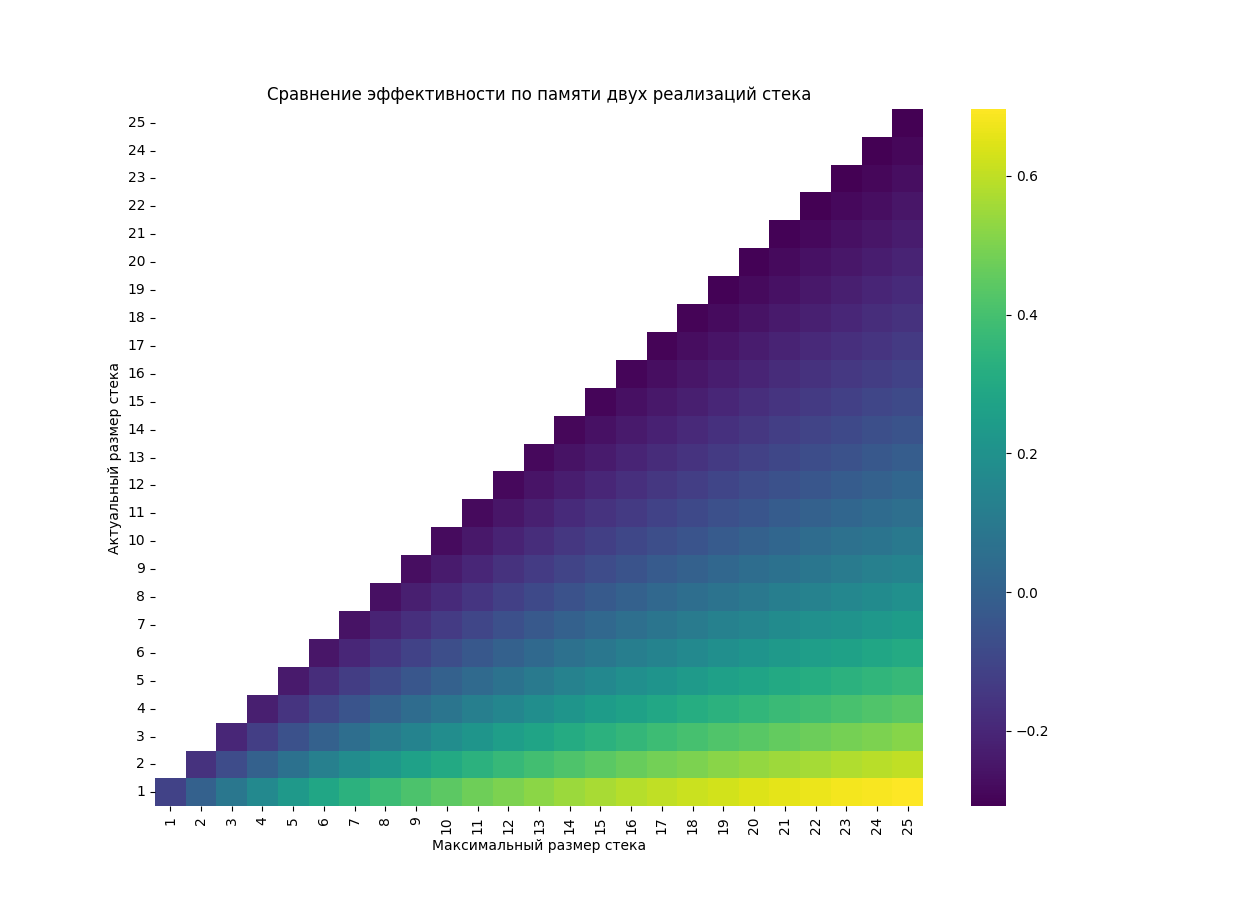
\includegraphics[width=\linewidth]{img/memgraph.png}
	\caption{Эффективность по памяти}
	\label{graph:mem}
\end{figure}

\clearpage

Ниже, на таблице \ref{table:mem}, представлена таблица сравнения эффективности по памяти стеков на основе массива и на основе списка. По результатам тестирования было выявлено, что при неполной заполненности стека (менее 50\%) эффективнее использовать реализацию на основе списка, так как для хранения стека потребуется меньший объем памяти.

\begin{table}
	\caption{Эффективность по памяти}
	\begin{center}
		\begin{tabular}{|c|c|c|c|c|}
			\hline
			Макс. размер & процент заполнения, \% & массив, байт & список, байт & эффективность, \% \\
			\hline
			10 & 10 & 104 & 40 & 62 \\
			10 & 50 & 104 & 104 & 0 \\
			10 & 70 & 104 & 136 & -31 \\
			1000 & 20 & 8024 & 3224 & 60 \\
			1000 & 40 & 8024 & 6424 & 20 \\
			1000 & 50 & 8024 & 8024 & 0 \\
			1000 & 60 & 8024 & 9624 & -20 \\
			\hline
		\end{tabular}
	\end{center}
	\label{table:mem}
\end{table}

\section{Вывод}

В результате эксперимента было получено, что операции со стеком, реализованном на основе массива в 7 раз эффективнее по времени, чем со стеком, реализованном на основе списка. Также было получено, что при заполненности стека менее 50\% стек на списке занимает меньше памяти, чем стек в массиве. В результате можно сделать вывод, что реализацию стека на списке выгодно использовать только в том случае, если необходимо получить стек, ограниченный лишь объемом оперативной памяти и если размер стека не превосходит половины от максимального.

\chapter{Контрольные вопросы}

\begin{enumerate}
	\item Что такое стек?
	
Стек --- это абстрактная структура данных, имеющая операции вставки и удаления элементов стека. Работает по принципу LIFO  --  последний пришёл - первый вышел. (работаем только с вершиной стека)

	\item Каким образом и сколько памяти выделяется под хранение стека при различной его реализации?
	
При реализации стека на статическом массиве память выделяется на стеке  (машинном)  единожды  и  никак  не  меняет  свой  размер  во  время работы программы. 

При реализации стека на динамическом массиве память выделяется в куче единожды в момент инициализации и впоследующем при нехватке свободного места в стеке. 

При реализации стека на связном списке память выделяется каждый раз при добавлении нового элемента в стек.

	\item Каким образом освобождается память при удалении элемента стека при различной реализации стека?
	
При реализации стека на статическом массиве память очищается при выходе из области видимости стека,  или проще говоря при завершении работы со стеком. 

При реализации стека на динамическом массиве память очищается при необходимости сжать стэк (уменьшить его вместимость до действительного размера), но этого можно не делать при частых и сбалансированных вставках и удалениях. 

При реализации стека на связном списке память очищается каждый раз при удалении элемента из стека.

	\item Что происходит с элементами стека при его просмотре? 
	
В  классической  реализации  стека  просмотр  (как  элементарное действие  над  стеком)  невозможен.  Для  просмотра  стека  необходимо использовать  дополнительную  структуру  данных  (не  обязательно  другой стек), переместив в неё последовательно все элементы из вершины стека. Тогда, складывая элементы обратно в стек, мы будем наблюдать их порядок при добавлении.

	\item Каким образом эффективнее реализовывать стек?
	
Эффективнее реализовывать стек на массиве, когда точно известно максимальное  число  элементов  в  нём,  а  размер  стека  зачастую  будет превышать  половину  от  максимального.  Но  если  не  представляется возможным  вычислить  это  число  заранее  или  зачастую  в  стеке  будет храниться  не  так  много  элементов  (менее  50\%),  то  эффективнее  будет использовать стек на связном списке.
\end{enumerate}
